\documentclass[11pt, a4paper]{article}

\usepackage{graphicx}
\usepackage[a4paper, margin=2.5cm]{geometry}
\usepackage{fontspec}
\usepackage[polish, english, bidi=basic, provide=*]{babel}
\babelprovide[import, onchar=ids fonts]{polish}
\babelfont{rm}{Noto Sans}

\usepackage{hyperref}
\usepackage{booktabs}
\usepackage{pdfpages}
\hypersetup{
    colorlinks=true,
    linkcolor=black,
    filecolor=black,      
    urlcolor=blue,
    pdftitle={Dokumentacja Projektowa - BYT},
    pdfpagemode=FullScreen,
}

\begin{document}
\begin{titlepage}
    \centering
    \vspace*{2cm}
    
    {\scshape\Large Przedmiot: BYT (Budowa i integracja systemów informatycznych) \par}
    \vspace{1.5cm}
    
    {\Huge\bfseries Dokumentacja Projektowa\par}
    \vspace{0.5cm}
    {\Large\bfseries System inteligentnego rezerwowania zasobów uniwersyteckich\par}
    
    \vspace{2cm}
    
    {\Large \textbf{Zespół projektowy:}\par}
    \vspace{0.5cm}
    {\large
        Tymur Katalnikov (Nr albumu: s33742) \par
        Zofia Michalska  (Nr albumu: s34264) \par
        Stanisław Pawłowski (Nr albumu: s28797) \par
        Ivan Syniuhin (Nr albumu: s24453) \par
    }
    
    \vspace{2cm}
    {\large \textbf{Zlecający (Klient):} \par}
    {\large Dział Informatyki Uczelni \par}
    
    \vfill
    
    {\large \today\par}
\end{titlepage}

\tableofcontents
\newpage

\section{Konwencje dokumentacyjne}
W niniejszym dokumencie przyjęto następujące zasady wyróżniania elementów tekstowych, aby ułatwić czytanie i analizę:
\begin{itemize}
    \item \textit{Kursywa} -- role użytkowników systemu (np. \textit{Wykładowca}, \textit{Student}, \textit{Administrator}).
    \item \textbf{Pogrubienie} -- elementy interfejsu graficznego oraz przyciski (np. kliknij \textbf{Zarezerwuj}, zakładka \textbf{Moje rezerwacje}).
    \item \texttt{Czcionka o stałej szerokości} -- nazwy klas, metod oraz zmiennych w diagramach i kodzie (np. klasa \texttt{Zasob}, metoda \texttt{znajdzDostepne()}).
\end{itemize}

\section{Koncepcja Projektowa}
\subsection{Opis systemu}
Projekt zakłada stworzenie aplikacji internetowej umożliwiającej \textit{Studentom} i \textit{Wykładowcom} rezerwowanie sal, laboratoriów lub sprzętu (np. gogli VR czy projektorów). 

System będzie integrować się z istniejącym planem zajęć uczelni, aby uniknąć nakładania się terminów. Wprowadzono również dodatkowe funkcjonalności, takie jak:
\begin{itemize}
    \item Automatyczne przypomnienia e-mail o zbliżających się rezerwacjach.
    \item Śledzenie statusu uszkodzonego sprzętu i wyłączanie go z dostępnej puli.
    \item Generowanie miesięcznych raportów wykorzystania zasobów dla \textit{Administratorów}.
\end{itemize}

\section{Projekt Architektury}
\subsection{Mały diagram klas (Ćwiczenie 2)}

\begin{figure}[h!]
    \centering
    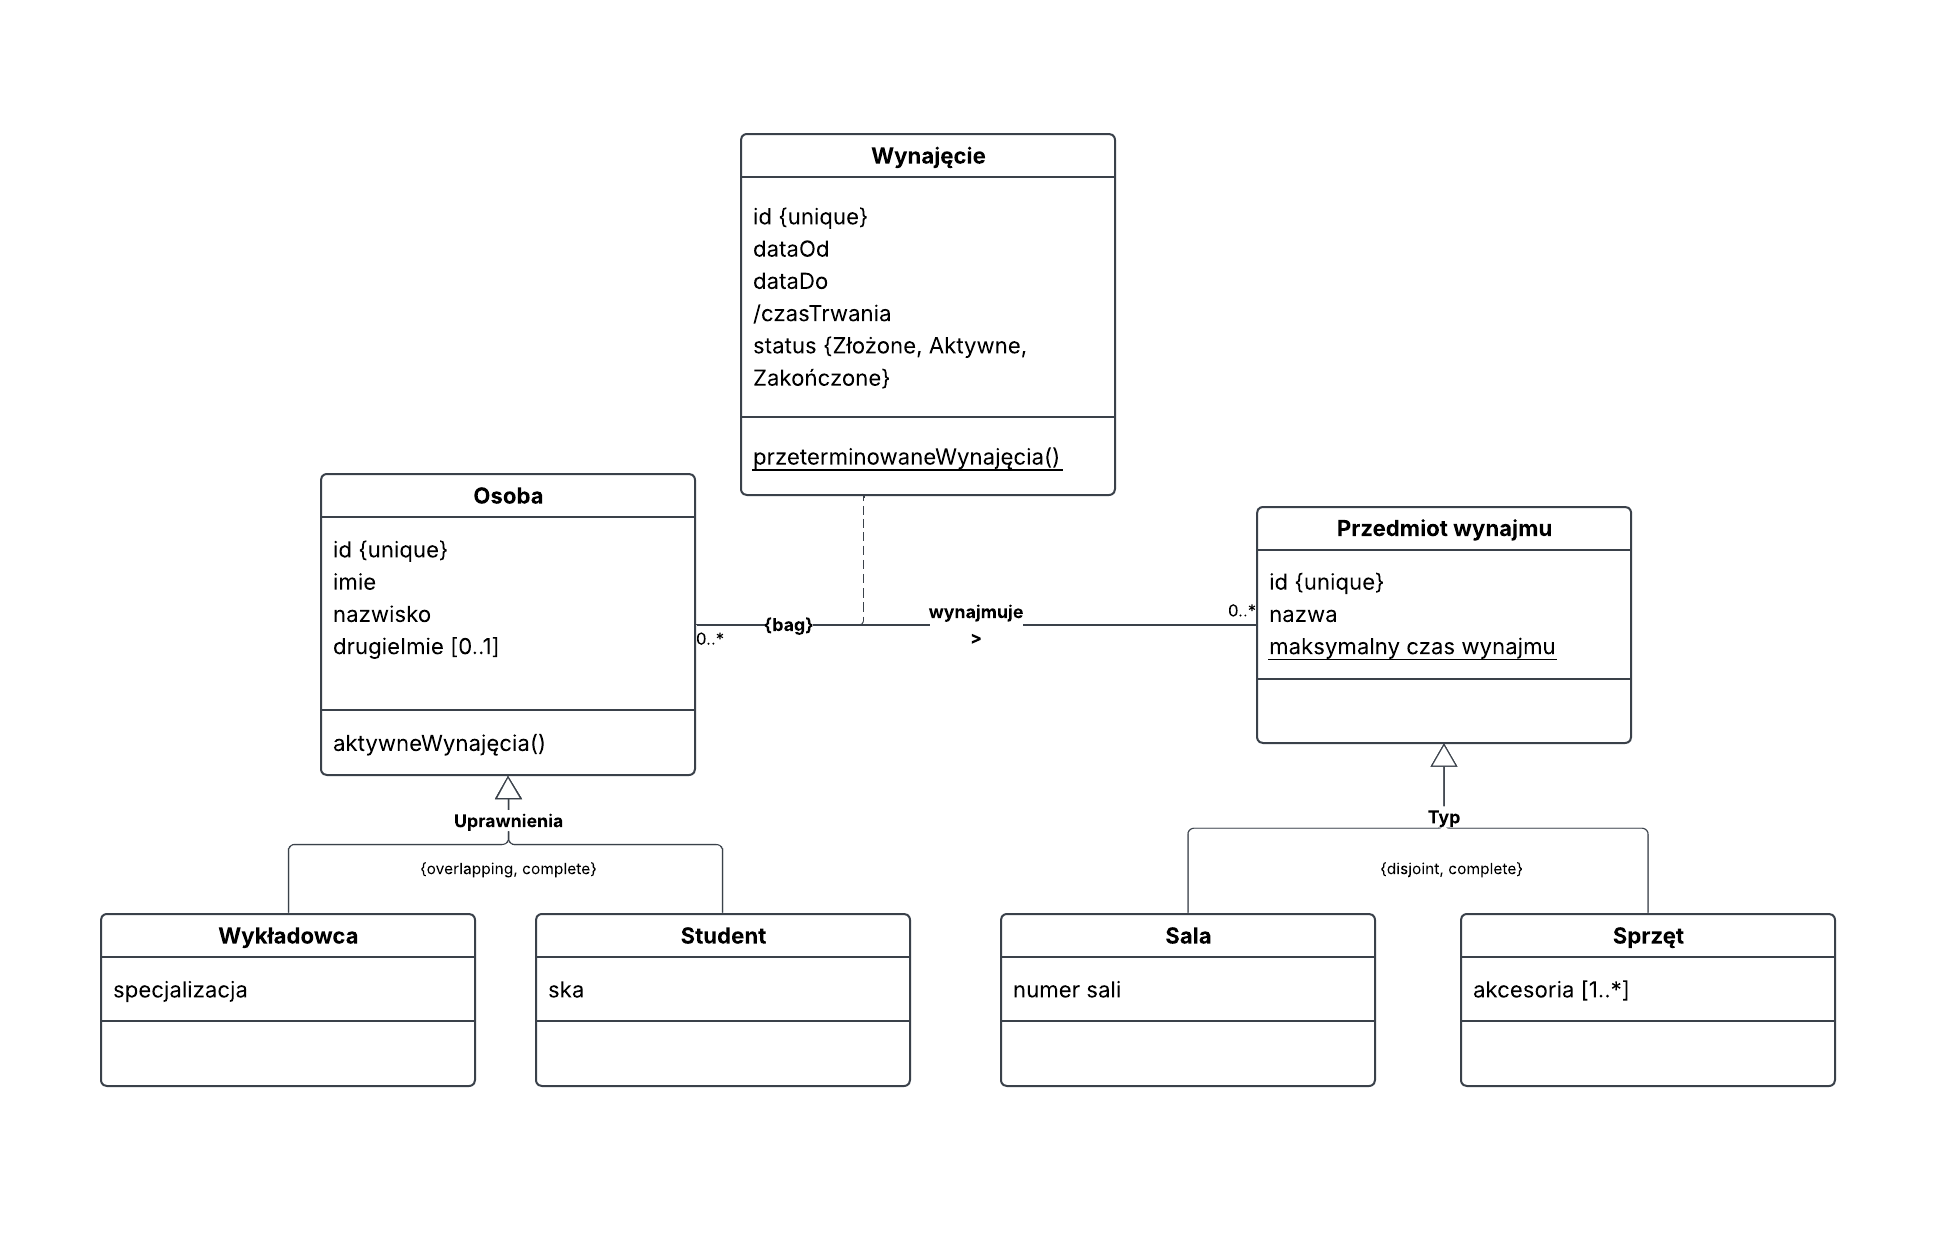
\includegraphics[width=0.8\textwidth]{BlankDiagram.png}
    \caption{Wstępny diagram klas obejmujący rezerwację zasobów przez użytkownika}
    \label{fig:diagram_klas}
\end{figure}

Jak widać na Rysunku \ref{fig:diagram_klas}, struktura opiera się na klasie asocjacji \texttt{Rezerwacja}, która łączy \texttt{Uzytkownika} z konkretnym \texttt{Zasobem}. Klasy te posiadają odpowiednie atrybuty i metody (np. \texttt{\_limitZasobow\_} czy \texttt{czasTrwania}), zgodnie z wymaganiami projektowymi.
\section{Wymagania Systemowe}

\subsection{Wymagania funkcjonalne}
\begin{itemize}
    \item Wymóg autoryzacji: dostęp do przeglądania i rezerwacji zasobów jest możliwy tylko dla zalogowanych użytkowników.
    \item System umożliwia \textit{Studentom} i \textit{Wykładowcom} rezerwację dostępnych sal i sprzętu w wybranym terminie.
    \item System automatycznie wysyła powiadomienia e-mail do użytkowników o zbliżającym się terminie rezerwacji.
    \item System pozwala \textit{Administratorom} na generowanie miesięcznych raportów wykorzystania zasobów.
\end{itemize}

\subsection{Wymagania niefunkcjonalne}
\begin{itemize}
    \item Aplikacja musi wspierać jednoczesne użytkowanie przez 2000 użytkowników bez odczuwalnych spadków wydajności.
    \item Czas ładowania strony głównej nie może przekroczyć 1.5 sekundy przy standardowych szybkościach transferu.
    \item Wszyscy użytkownicy muszą korzystać z 2FA podczas autentykacji.
    \item Wszystkie dane osobowe muszą być szyfrowane standardem AES-256.
    \item W przypadku awarii systemu, czas przywrócenia pełnej sprawności wraz z danymi nie powinien przekroczyć 24 godzin.
\end{itemize}

\newpage
\section{Diagram Przypadków Użycia}
Poniżej przedstawiono diagram przypadków użycia oraz zestawienie aktorów i przypadków wygenerowane w programie Enterprise Architect.

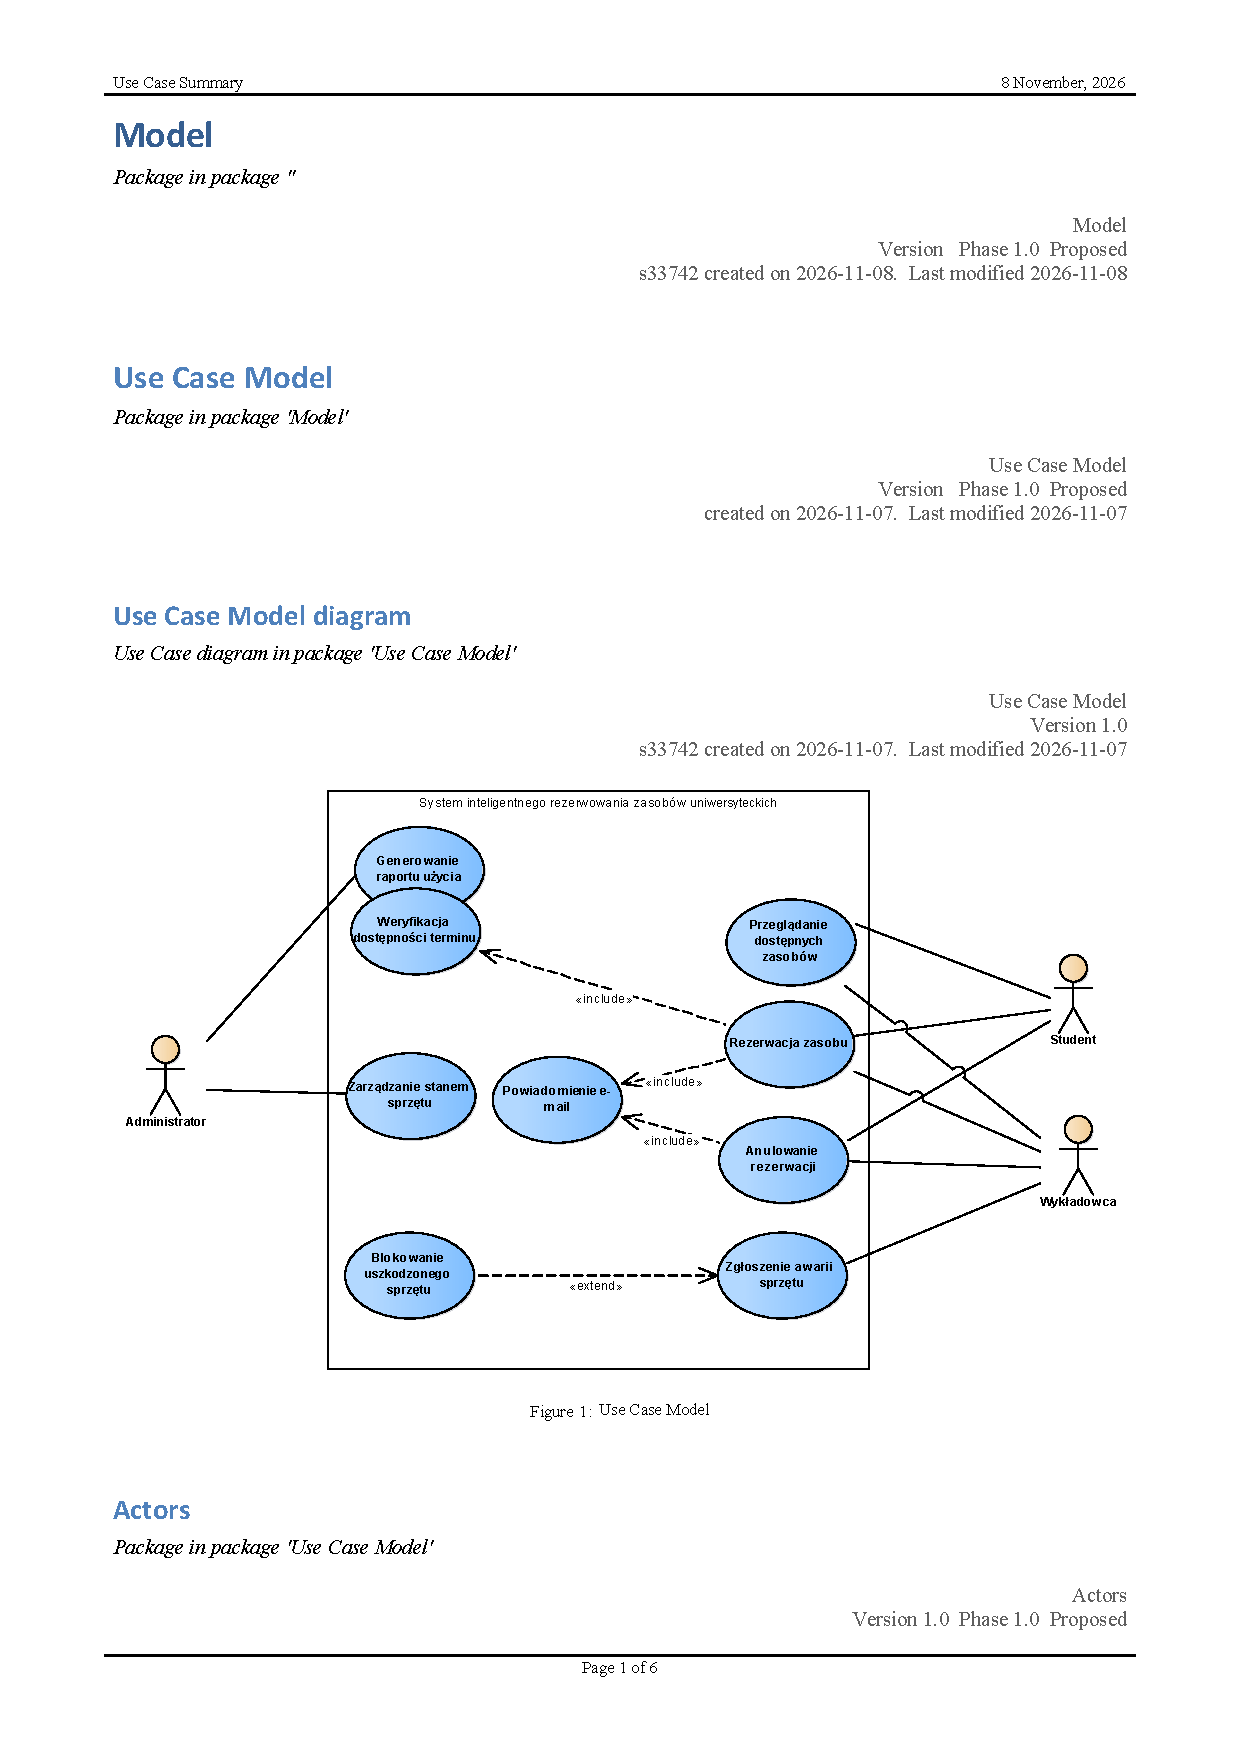
\includepdf[pages=-]{diagram_uc.pdf}
\listoffigures
\newpage
\end{document}